\begin{notechapter}
\chapter{Conditional Random Fields}\label{ch:crf}
\chaptersubtitle{A discriminative model of tag sequences, normalized over the whole sequence}

\begin{chapterintro}
An HMM models how words are generated from tags, so every feature of the input must be
part of the generative story: adding ``the word ends in \emph{-ing}'' or ``the next word is \emph{to}'' would
require modelling those events too, with independence assumptions that do not hold. A
conditional random field (CRF) models $p(y\mid x)$ directly. It scores a tag sequence with arbitrary
features of the whole input, adds transition scores between neighbouring tags, and
normalizes over all tag sequences at once. The Viterbi and forward algorithms of
\cref{ch:hmm-viterbi} carry over unchanged, and the gradient of the log-likelihood has a
simple form: observed feature counts minus expected ones. You will learn
\begin{itemize}[nosep]
  \item the linear-chain CRF, with feature weights or with neural emission scores;
  \item that the conditional distribution of an HMM is a special case;
  \item how $Z(x)$ is computed by the forward algorithm and the best sequence by Viterbi;
  \item the gradient of the log-likelihood, why it needs the forward--backward marginals, and
        why automatic differentiation of the forward algorithm computes it;
  \item a worked example checked by enumeration, and the BiLSTM--CRF tagger.
\end{itemize}
\prerequisites{\cref{ch:hmm-viterbi}; generative and discriminative models
(\cref{ch:generative-discriminative}); softmax regression (\cref{ch:bigram-models}).}
\end{chapterintro}

\section{The linear-chain CRF}\label{crf:sec:definition}

\begin{definition}[Linear-chain CRF]\label{crf:def:crf}
Let $x$ be an input sequence of length $T$ and $y = (y_1,\dots,y_T)$ a tag sequence, $y_t\in\{1,\dots,K\}$, with a fixed start
symbol $y_0$. Given score functions $\psi_t(j, k; x)$, the \emph{linear-chain CRF} is
\[
  p(y\mid x) = \frac{\exp S(x, y)}{Z(x)},\qquad S(x, y) = \sum_{t=1}^T\psi_t(y_{t-1}, y_t; x),\qquad Z(x) = \sum_{y'}\exp S(x, y'),
\]
where the sum defining $Z(x)$, the \emph{partition function}, runs over all $K^T$ tag sequences.
\end{definition}

The model is softmax regression (\cref{ch:bigram-models}) over the $K^T$ sequences, with a score that
decomposes into terms involving two neighbouring tags. Each term may depend on the
\emph{whole} input $x$ and on the position $t$. Two parameterizations are common.
\begin{itemize}
  \item \emph{Feature weights} (Lafferty, McCallum and Pereira, \emph{Conditional Random Fields:
        Probabilistic Models for Segmenting and Labeling Sequence Data}, 2001):
        $\psi_t(j, k; x) = \theta^\top f(j, k, x, t)$, with hand-designed indicator features such as $[j = \mathrm D][k = \mathrm N]$ (a transition),
        $[k = \mathrm N][x_t\text{ ends in -s}]$, $[k = \mathrm V][x_{t-1} = \text{to}]$ or $[k = \mathrm N][x_t\text{ is capitalized}]$. The features overlap and are strongly
        dependent, which is harmless for a conditional model.
  \item \emph{Neural emissions}: $\psi_t(j, k; x) = A_{jk} + U_{t,k}(x)$, where $U_t(x)\in\R^K$ is computed by a network from the whole
        sentence, typically a bidirectional LSTM (\cref{sequence-models:sec:bidirectional}), and $A$ is a learned
        $K\times K$ transition matrix (Huang, Xu and Yu, \emph{Bidirectional LSTM-CRF Models for Sequence
        Tagging}, 2015; Lample et al., \emph{Neural Architectures for Named Entity Recognition},
        2016).
\end{itemize}

\begin{figure}[ht]
\centering
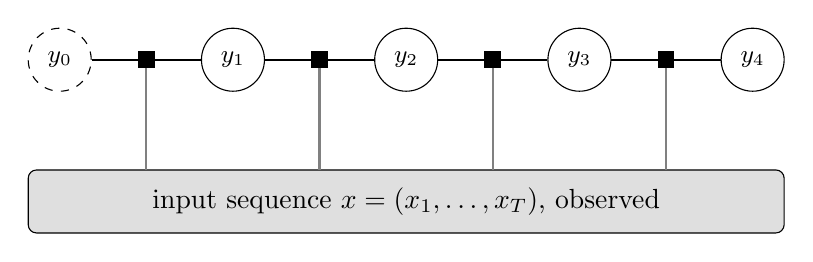
\begin{tikzpicture}[
  v/.style={draw, circle, minimum size=8mm, inner sep=0pt, font=\small},
  fac/.style={draw, fill=black, minimum size=2mm, inner sep=0pt},
  ln/.style={thick}]
  \node[draw, rounded corners=3pt, fill=gray!25, minimum width=9.6cm, minimum height=8mm] (x) at (4.4,-1.8) {input sequence $x = (x_1,\dots,x_T)$, observed};
  \node[v, dashed] (y0) at (0,0) {$y_0$};
  \foreach \t in {1,2,3,4} \node[v] (y\t) at (2.2*\t,0) {$y_{\t}$};
  \foreach \t/\p in {1/0,2/1,3/2,4/3} {
    \node[fac] (f\t) at (2.2*\t-1.1,0) {};
    \draw[ln] (y\p) -- (f\t) -- (y\t);
    \draw[ln, gray] (f\t) -- (2.2*\t-1.1,-1.4);
  }
\end{tikzpicture}
\caption{A linear-chain CRF as a factor graph. Each black square is a factor $\exp\psi_t(y_{t-1}, y_t; x)$, which links two
neighbouring tags and may read the whole input. The input is conditioned on, not modelled.}
\label{crf:fig:graph}
\end{figure}

\begin{proposition}[HMMs are CRFs]\label{crf:prop:hmm}
For an HMM (\cref{hmm-viterbi:def:hmm}), $p(y\mid x)$ is a linear-chain CRF with
$\psi_1(y_0, k; x) = \log\pi_k + \log B_k(x_1)$ and $\psi_t(j, k; x) = \log A_{jk} + \log B_k(x_t)$ for $t\geq2$.
\end{proposition}

\begin{proof}
With these scores, $\exp S(x, y) = p(x, y)$. Hence $Z(x) = \sum_yp(x, y) = p(x)$, and the
ratio $\exp S(x, y)/Z(x)$ is $p(y\mid x)$.
\end{proof}

The converse fails: a CRF's scores need not be log-probabilities, and they may depend on any
part of $x$. The CRF family is the larger one, and training it maximizes the conditional likelihood,
the quantity that matters for tagging (\cref{ch:generative-discriminative}). The price is that its
training is no longer counting.

\section{Inference: the partition function and the best sequence}\label{crf:sec:inference}

The forward and Viterbi recursions of \cref{ch:hmm-viterbi} only used the decomposition of the
score into neighbouring pairs, so they apply with $\exp\psi_t$ in place of $A_{jk}B_k(x_t)$. In log space, with
$a_t(k) = \log\sum_{y_{1:t-1}}\exp S_{1:t}(x, y_{1:t-1}, y_t = k)$ (the log of the summed scores of the prefixes ending in $k$),
\begin{gather*}
  a_1(k) = \psi_1(y_0, k; x),\qquad a_t(k) = \operatorname{logsumexp}_j\bigl(a_{t-1}(j) + \psi_t(j, k; x)\bigr),\\
  \log Z(x) = \operatorname{logsumexp}_ka_T(k),
\end{gather*}
and Viterbi replaces logsumexp by max, giving $\arg\max_yp(y\mid x) = \arg\max_yS(x, y)$ in $O(TK^2)$, without computing $Z(x)$.

\begin{pitfall}[Global versus local normalization]
A CRF normalizes once, over whole sequences. A tempting alternative normalizes at every
step, $p(y\mid x) = \prod_tp(y_t\mid y_{t-1}, x)$, with a softmax over $y_t$ (a maximum-entropy Markov model). Such models suffer from the
\emph{label bias} problem identified by Lafferty et al.: each step must distribute exactly one unit of
probability among the successors of $y_{t-1}$, so a state with few successors passes its mass on
whatever the current word says, and evidence later in the sentence cannot lower the
probability of an early choice. Global normalization lets the scores of all the positions compete,
which is why the partition function is over sequences and not over single tags.
\end{pitfall}

\section{Training: observed minus expected features}\label{crf:sec:training}

The conditional log-likelihood of a training pair $(x, y)$ is $\log p(y\mid x) = S(x, y) - \log Z(x)$. For the
feature-weight parameterization, $S(x, y) = \theta^\top F(x, y)$ with the global feature vector $F(x, y) = \sum_tf(y_{t-1}, y_t, x, t)$.

\begin{proposition}[Gradient of the log-likelihood]\label{crf:prop:gradient}
\begin{align*}
  \nabla_\theta\log p(y\mid x) &= F(x, y) - \E_{y'\sim p(\cdot\mid x)}\bigl[F(x, y')\bigr]\\
  &= F(x, y) - \sum_{t=1}^T\sum_{j,k}p(y'_{t-1} = j,\ y'_t = k\mid x)\,f(j, k, x, t) .
\end{align*}
The negative log-likelihood is convex in $\theta$.
\end{proposition}

\begin{proof}
$\nabla_\theta\log Z = \frac1Z\sum_{y'}e^{\theta^\top F(x,y')}F(x, y') = \sum_{y'}p(y'\mid x)F(x, y')$, the derivative of a log-sum-exp being the
softmax-weighted average of the derivatives of its arguments. Since $F(x, y')$ is a sum over $t$ of
terms that depend on $(y'_{t-1}, y'_t)$ only, its expectation needs only the pairwise marginals. Convexity: $\log Z$
is a log-sum-exp of linear functions of $\theta$, hence convex, and $-S(x, y)$ is linear.
\end{proof}

At the optimum (without regularization), the expected count of every feature under the model
equals its count in the data, the same moment-matching that made softmax regression
reproduce the bigram counts (\cref{bigram-models:sec:convergence}). The pairwise marginals are
computed by the forward--backward recursions,
\[
  p(y_{t-1} = j,\ y_t = k\mid x) = \frac{\exp\bigl(a_{t-1}(j) + \psi_t(j, k; x) + b_t(k)\bigr)}{Z(x)},
\]
with the backward quantities $b_t(k) = \operatorname{logsumexp}_l\bigl(\psi_{t+1}(k, l; x) + b_{t+1}(l)\bigr)$, $b_T(k) = 0$. Each training step costs
$O(TK^2)$ per sentence, and the convex objective (with an $L_2$ penalty) is minimized by L-BFGS or
stochastic gradient descent. For a neural CRF, the loss $\log Z(x) - S(x, y)$ is computed with the forward
recursion and differentiated by backpropagation; reverse-mode differentiation through the
log-sum-exp recursion computes exactly the forward--backward marginals (Eisner, \emph{Inside-Outside
and Forward-Backward Algorithms Are Just Backprop}, 2016), so no backward recursion has to be
written.

\begin{example}[Two tags, three positions]\label{crf:ex:small}
Tags D and N, $T = 3$, neural-style scores $\psi_t(j, k) = A_{jk} + U_{t,k}$ with start scores $\psi_1(y_0, k) = s_k + U_{1,k}$:
\[
  U = \begin{bmatrix}1 & 0\\ 0 & 1\\ 0.5 & 0.5\end{bmatrix},\qquad
  A = \begin{bmatrix}-1 & 2\\ 0.5 & 0\end{bmatrix},\qquad s = (0.5,\ 0),
\]
where the rows of $U$ are the positions $t$ and its columns the tags D, N, and $A_{jk}$ is the score of the
transition from $j$ to $k$, in the same order.
\emph{Scores.} For instance $S(\mathrm{D,N,D}) = (0.5 + 1) + (2 + 1) + (0.5 + 0.5) = 5.5$. The eight sequences have scores $0, 3, 5.5, 5, 0, 3, 2, 1.5$
(in the order DDD, DDN, DND, DNN, NDD, NDN, NND, NNN).

\emph{Forward.} $a_1 = (1.5, 0)$; $a_2(\mathrm D) = \operatorname{logsumexp}(1.5 - 1,\ 0 + 0.5) + 0 = 1.1931$, $a_2(\mathrm N) = \operatorname{logsumexp}(1.5 + 2,\ 0 + 0) + 1 = 4.5298$;
$a_3 = (5.5377, 5.2630)$; $\log Z = \operatorname{logsumexp}(5.5377, 5.2630) = 6.1029$, $Z = 447.15$, which the sum of $e^S$ over the eight sequences
confirms.

\emph{Probabilities and decoding.} $p(\mathrm{DND}\mid x) = e^{5.5}/447.15 = 0.547$ and $p(\mathrm{DNN}\mid x) = 0.332$; Viterbi returns DND.

\emph{Gradient.} For the observed sequence $y = \mathrm{DNN}$, the loss is $\log Z - S(x, y) = 6.1029 - 5 = 1.1029$. Its gradient with
respect to the transition matrix is (expected $-$ observed) transition counts:
\[
  \nabla_A\bigl(-\log p(y\mid x)\bigr) = \underbrace{\begin{bmatrix}0.0516 & 0.9690\\ 0.6109 & 0.3685\end{bmatrix}}_{\text{expected counts}}
  - \underbrace{\begin{bmatrix}0 & 1\\ 0 & 1\end{bmatrix}}_{\text{observed (D}\to\text{N, N}\to\text{N)}}
  = \begin{bmatrix}0.0516 & -0.0310\\ 0.6109 & -0.6315\end{bmatrix} .
\]
A gradient step raises $A_{\mathrm{NN}}$ and lowers $A_{\mathrm{ND}}$, moving probability from DND to the observed DNN.
\end{example}

The forward recursion as a differentiable loss in PyTorch; automatic differentiation gives the
gradient of the example, and the result agrees with enumeration:
\begin{lstlisting}[language=Python]
import torch

def crf_nll(U, A, s, y):
    """U: (T, K) emission scores, A: (K, K) transitions, s: (K,) start scores,
       y: list of T tags. Returns log Z(x) - S(x, y)."""
    a = s + U[0]                                        # a_1
    for t in range(1, U.shape[0]):
        a = torch.logsumexp(a[:, None] + A, dim=0) + U[t]
    log_Z = torch.logsumexp(a, dim=0)
    score = s[y[0]] + U[0, y[0]] + sum(A[y[t - 1], y[t]] + U[t, y[t]]
                                       for t in range(1, len(y)))
    return log_Z - score

U = torch.tensor([[1.0, 0.0], [0.0, 1.0], [0.5, 0.5]])
A = torch.tensor([[-1.0, 2.0], [0.5, 0.0]], requires_grad=True)
loss = crf_nll(U, A, torch.tensor([0.5, 0.0]), [0, 1, 1])   # y = D, N, N
loss.backward()            # loss = 1.1029; A.grad = expected - observed counts
\end{lstlisting}

\section{HMM or CRF?}\label{crf:sec:comparison}

\begin{center}\small
\begin{tabular}{p{0.2\textwidth}p{0.34\textwidth}p{0.36\textwidth}}
 & \textbf{HMM} & \textbf{linear-chain CRF}\\\hline
models & $p(x, y)$ (generative) & $p(y\mid x)$ (discriminative)\\
input features & one word per tag, through $B_k(x_t)$ & any features of the whole input\\
supervised training & counting, closed form & convex optimization, forward--backward at each step\\
unlabelled data & Baum--Welch (EM) & not directly usable\\
decoding & Viterbi & Viterbi
\end{tabular}
\end{center}
With little data, the generative HMM can be competitive (\cref{ch:generative-discriminative});
with enough data and informative features, the CRF is usually more accurate, which made it the
standard tagger before neural networks, and the layer placed on top of them afterwards.

\begin{chaptersummary}
\begin{itemize}
  \item A linear-chain CRF is a softmax over tag sequences with a score $S(x, y) = \sum_t\psi_t(y_{t-1}, y_t; x)$ that may use the whole
        input; it is normalized globally, which avoids the label bias of per-step normalization.
  \item The conditional distribution of an HMM is a CRF with log-probability scores; CRFs are more
        general.
  \item $Z(x)$ is computed by the forward recursion in log space, the best sequence by Viterbi, both in
        $O(TK^2)$.
  \item $\nabla_\theta\log p(y\mid x) = F(x, y) - \E_{p(y'\mid x)}[F(x, y')]$: observed minus expected features, with pairwise marginals from
        forward--backward; the objective is convex in the feature weights.
  \item A BiLSTM--CRF computes the emission scores with a bidirectional LSTM and learns a transition
        matrix; backpropagation through the forward recursion gives the gradient.
\end{itemize}
\end{chaptersummary}

\section*{Exercises}
\addcontentsline{toc}{section}{Exercises}

\begin{exercise}\label{crf:exr:1}
In \cref{crf:ex:small}, compute $S$ for the eight sequences and check that $\sum e^S = 447.15$.
\solutionlink{crf:exr:1}
\end{exercise}

\begin{exercise}\label{crf:exr:2}
Show that adding a constant $c$ to every entry of $A$ does not change $p(y\mid x)$ for sequences of a fixed length $T$. What
does this imply for the gradient with respect to $A$ (check it on the example)?
\solutionlink{crf:exr:2}
\end{exercise}

\begin{exercise}\label{crf:exr:3}
For $T = 1$, show that the CRF is multinomial logistic regression on the scores $\psi_1(y_0, k; x)$, and that
\cref{crf:prop:gradient} gives the gradient $p - y$ of \cref{bigram-models:sec:gradient}.
\solutionlink{crf:exr:3}
\end{exercise}

\begin{exercise}\label{crf:exr:4}
Prove the formula for the pairwise marginals $p(y_{t-1} = j, y_t = k\mid x)$ from the definitions of $a_{t-1}$ and $b_t$.
\solutionlink{crf:exr:4}
\end{exercise}

\begin{exercise}\label{crf:exr:5}
A tagger computes the emission scores $U_t(x)$ with a bidirectional LSTM and predicts each tag
independently with a softmax over $U_t(x)$. What can a CRF layer on top of it add, given that the
LSTM already sees the whole sentence?
\solutionlink{crf:exr:5}
\end{exercise}
\end{notechapter}
